\documentclass[conference]{IEEEtran}
\IEEEoverridecommandlockouts
\usepackage{cite}
\usepackage{amsmath,amssymb,amsfonts}
\usepackage{graphicx}
\graphicspath{{figures/}}
\usepackage{booktabs}
\usepackage{array}
\usepackage{url}
\usepackage{xcolor}
\usepackage{hyperref}
\hypersetup{colorlinks=true,linkcolor=black,citecolor=black,urlcolor=blue}

\begin{document}

\title{What Local Costs: A Paired Evaluation of a Single-GPU Financial RAG
Pipeline Against a Published API-Based System}

\author{
\IEEEauthorblockN{Haroon M. Bilal}
\IEEEauthorblockA{\textit{Department of Computer Science} \\
\textit{University of Management and Technology}\\
Lahore, Pakistan \\
haroonmbilal007@gmail.com}
\and
\IEEEauthorblockN{Muhammad Bin Sarwar}
\IEEEauthorblockA{\textit{Department of Computer Science} \\
\textit{University of Management and Technology}\\
Lahore, Pakistan \\
muhammad.b.sarwar8@gmail.com}
}

\maketitle

\begin{abstract}
Retrieval-augmented generation (RAG) systems for financial filings are usually
built on paid APIs and evaluated only on the quality of the final written
answer, which leaves two questions unanswered: how much of a system's
performance comes from retrieval rather than generation, and what is lost by
running the whole pipeline locally. We build FinRAG, a RAG pipeline over 497
S\&P~500 10-K filings that runs entirely on one 12\,GB laptop GPU with no paid
services, fine-tuning a 33M-parameter embedder, a cross-encoder reranker and
three generators (3B--7B) with QLoRA. We then evaluate it against HDRR
\cite{hdrr2026}, a published 2026 system on the same benchmark, under an
unusually strict protocol: the same 258 held-out queries, HDRR's own GPT-4.1
judge, rubric and prompt verbatim, and a paired bootstrap over per-query
scores. We first validate our grader by re-scoring 40 of HDRR's own published
answers, reproducing them at 90\% exact agreement, 100\% within one point and
$r=0.993$. FinRAG scores 6.02/10 against HDRR's 7.63 (95\% CI
$[-2.08,-1.13]$), and is statistically indistinguishable from one of their five
published configurations. Supplying gold evidence raises FinRAG to 6.70, which
decomposes the gap into 0.67 attributable to retrieval and 0.93 to generator
capacity. On retrieval --- which HDRR does not report --- FinRAG reaches
NDCG@10 0.599 on filings never seen in training. Finally, we replace HDRR's
per-query LLM ticker extraction with a dictionary built from public SEC
company-name data: it routes 90.8\% of queries at 99.3\% precision and agrees
with their LLM router on 100\% of the 232 queries where both commit, at zero
inference cost. We argue that the useful contribution of local financial RAG is
not higher answer quality but a measured account of what quality costs.
\end{abstract}

\begin{IEEEkeywords}
retrieval-augmented generation, dense retrieval, document routing, financial
NLP, question answering, QLoRA, LLM-as-judge, reproducibility
\end{IEEEkeywords}

\section{Introduction}
Financial analysts answer narrow, factual questions by reading long regulatory
filings: how a company's segment revenue moved between two years, what a
specific accounting policy says, which risks were disclosed. Large language
models are prone to fabricating such figures, and retrieval-augmented
generation (RAG)~\cite{lewis2020rag} mitigates this by grounding the answer in
retrieved passages.

Published financial RAG systems share two properties that limit what can be
learned from them. First, they depend on paid APIs --- typically for
embeddings, for query or entity rewriting, and for generation --- so their
reported quality is partly a statement about the budget behind them. Second,
they are evaluated end to end, usually by an LLM judge scoring the final
answer. An end-to-end score cannot say whether a wrong answer came from
retrieving the wrong passage or from reasoning badly over the right one, and
the systems that report it generally publish no retrieval metrics at all, even
when the benchmark supplies gold evidence.

This paper takes the opposite position deliberately. We build a pipeline
constrained to one consumer GPU and no paid inference, measure each stage
separately, and then compare the whole system against a published API-based
system on that system's own terms. The comparison is a loss, and we report it
as one; the contribution is in what the loss can be decomposed into.

Our contributions are:

\begin{itemize}
\item \textbf{A paired evaluation protocol against a published system, with
grader validation.} HDRR~\cite{hdrr2026} releases per-query judge scores, which
allows a paired comparison on identical questions rather than a comparison of
two aggregates. We restrict to queries whose filings never appear in our
training data, re-use their judge, rubric and prompt verbatim, and first
demonstrate that our grading harness reproduces their published scores
($r=0.993$). We are not aware of prior financial RAG work that validates its
LLM judge against a baseline's own published outputs before comparing to them.

\item \textbf{A decomposition of the gap to a frontier-API system.} By
evaluating the same generator on retrieved and on gold evidence, we separate
the 1.61-point deficit into 0.67 from retrieval and 0.93 from generator
capacity --- a distinction that an end-to-end score cannot express, and which
HDRR cannot compute for its own system.

\item \textbf{Document routing without an LLM.} HDRR extracts a company ticker
with one LLM call per query. We replace it with a dictionary derived from
public SEC company-name data plus an acronym stoplist, which recovers most of
that capability at zero cost and agrees with their router on every query where
both commit.

\item \textbf{Retrieval metrics on FinDER under a leakage-free protocol},
including graded multi-chunk relevance labels built by a coverage criterion
that is stable across chunk sizes, and a filing-level train/test split.
\end{itemize}

\section{Related Work}
\textbf{Dense retrieval.} Dense Passage Retrieval~\cite{karpukhin2020dpr}
established contrastively trained dual encoders over sparse baselines such as
BM25~\cite{robertson2009bm25}. ColBERT~\cite{khattab2020colbert} trades cost
for accuracy via late interaction; Sentence-BERT~\cite{reimers2019sbert}
introduced siamese sentence embeddings. Contriever~\cite{izacard2022contriever},
E5~\cite{wang2022e5}, GTR~\cite{ni2022gtr} and the BGE
family~\cite{xiao2023bge} are strong general-purpose retrievers.
BEIR~\cite{thakur2021beir} is the standard zero-shot comparison suite. We build
on BGE because its small variant (33M parameters) is the largest model that
leaves room for a 7B generator on a single 12\,GB card.

\textbf{Reranking and fusion.} Cross-encoder
rerankers~\cite{nogueira2019passage} re-score a first-stage candidate list.
Reciprocal Rank Fusion~\cite{cormack2009rrf} merges dense and sparse rankings.
HyDE~\cite{gao2022hyde} rewrites the query into a hypothetical document; we do
not use it, as it requires generation at retrieval time.

\textbf{Parameter-efficient fine-tuning.} LoRA~\cite{hu2021lora} trains low-rank
updates; QLoRA~\cite{dettmers2023qlora} adds 4-bit quantization so a 7B model
fits on consumer hardware. Our generators are
Qwen2.5~\cite{qwen2024}, Llama-3.2~\cite{touvron2023llama} and
Mistral~\cite{jiang2023mistral}.

\textbf{Financial NLP and benchmarks.} FinBERT~\cite{araci2019finbert} and
BloombergGPT~\cite{wu2023bloomberggpt} are domain-adapted language models;
FinQA~\cite{chen2021finqa} targets numerical reasoning.
FinDER~\cite{finder2025} is the retrieval-oriented benchmark we use, built on
S\&P~500 10-K filings with gold evidence passages. Its own paper reports
retrieval as RAGAS~\cite{es2023ragas} Context Recall rather than rank-based
metrics.

\textbf{The systems we compare against.} Cheng \textit{et
al.}~\cite{basepaper2026} built a financial RAG system on FinDER with
off-the-shelf embeddings, a cross-encoder reranker and a paid LLM for query
rewriting and generation, evaluated with an LLM judge. Their follow-up,
HDRR~\cite{hdrr2026}, adds hybrid document-routed retrieval, in which an LLM
first extracts the target company and retrieval is then confined to that
company's filing. HDRR is our primary comparison point: it is recent, it uses
the same benchmark, and --- critically --- it publishes per-query judge scores,
which makes a paired comparison possible. Neither paper reports retrieval
metrics.

\textbf{LLM-as-judge.} Automatic judging with a strong
model~\cite{zheng2023judge} is now standard for open-ended generation, with
known caveats including position bias and self-preference. We address the most
relevant one here --- that the judge and the baseline's generator come from the
same model family --- in Section~\ref{sec:limits}.

\section{Dataset and Evidence Alignment}
\label{sec:data}
We use FinDER~\cite{finder2025}: 497 S\&P~500 10-K filings and 5{,}703
questions, each with a gold answer and one or more \emph{reference} passages
quoted from the filing. Questions are short and heavily abbreviated
(e.g.\ ``Delta in CBOE Data \& Access Solutions rev from 2021-23''), and a
substantial minority require a small arithmetic step.

\textbf{Chunking.} We parse each filing to text and split it into chunks of 448
tokens with 112 tokens of overlap, measured \emph{in the retriever's own
tokenizer} rather than in words. This matters: a chunk defined in words can
exceed the encoder's 512-token limit and be silently truncated at encoding
time. The result is 181{,}867 chunks.

\textbf{Graded, filing-restricted relevance labels.} FinDER gives evidence as
raw text, not chunk identifiers, so relevance labels must be induced. A
single-best-match criterion is both too coarse (evidence spans several chunks;
mean 2.18 in our labels) and too permissive (10-K boilerplate is near-identical
across companies, so a global match frequently lands in the wrong filing). We
therefore resolve each question to exactly one filing first, by summed TF--IDF
similarity over its references, and then select chunks \emph{within that filing}
by greedy union coverage: chunks are added until their union covers 80\% of the
reference's token multiset. The chunk contributing the largest share is graded
2 (primary evidence), others 1 (supporting).

Union coverage is a property of the evidence rather than of the chunk size, so
the threshold does not need re-tuning when chunking changes --- unlike a
per-chunk overlap threshold, which must be lowered as chunks shrink. This
yields labels for 5{,}303 of 5{,}703 questions (93.0\%), with 99.2\% of
references reaching the coverage target and, by construction, no question whose
gold spans more than one filing. Table~\ref{tab:dataset} summarizes the corpus.

\begin{table}[t]
\caption{FinDER as processed in this work.}
\label{tab:dataset}
\centering
\small
\begin{tabular}{ll}
\toprule
Property & Value \\
\midrule
Filings (10-K) & 497 \\
Questions & 5{,}703 \\
Chunks (448 tokens, 112 overlap) & 181{,}867 \\
Questions with induced labels & 5{,}303 (93.0\%) \\
Relevant chunks per question (mean / median) & 2.18 / 2 \\
References reaching 80\% coverage & 99.2\% \\
Train / test filings & 392 / 98 \\
Train / test questions & 4{,}215 / 1{,}088 \\
\bottomrule
\end{tabular}
\end{table}

\textbf{Leakage-free splitting.} We split at the \emph{filing} level, not the
question level: 392 filings (4{,}215 questions) for training and 98 filings
(1{,}088 questions) for evaluation. Because many FinDER questions target the
same filing, a question-level split would let a retriever memorize the exact
passages it is later tested on. Retrieval at inference still searches the full
181{,}867-chunk corpus; only training is restricted.

\textbf{Label audit.} Our filing-resolution step includes an override that
trusts an explicitly named ticker over the TF--IDF result. Ticker strings
collide with financial vocabulary --- \texttt{IP} is also intellectual
property, \texttt{CF} cash flow, \texttt{NI} net income --- so we audited the
labels for questions matching that failure mode exactly. On the test split,
zero questions are affected. On the training split, 166 (3.9\%) match the
pattern, but their selected gold chunks cover the query text as well as any
other question's (0.477 versus 0.450), indicating genuine mentions of those
companies rather than mislabelling.

\section{Method}
Fig.~\ref{fig:pipeline} shows the pipeline. Four components are trained or
constructed by us; none of them call an external service.

\begin{figure}[t]
\centering
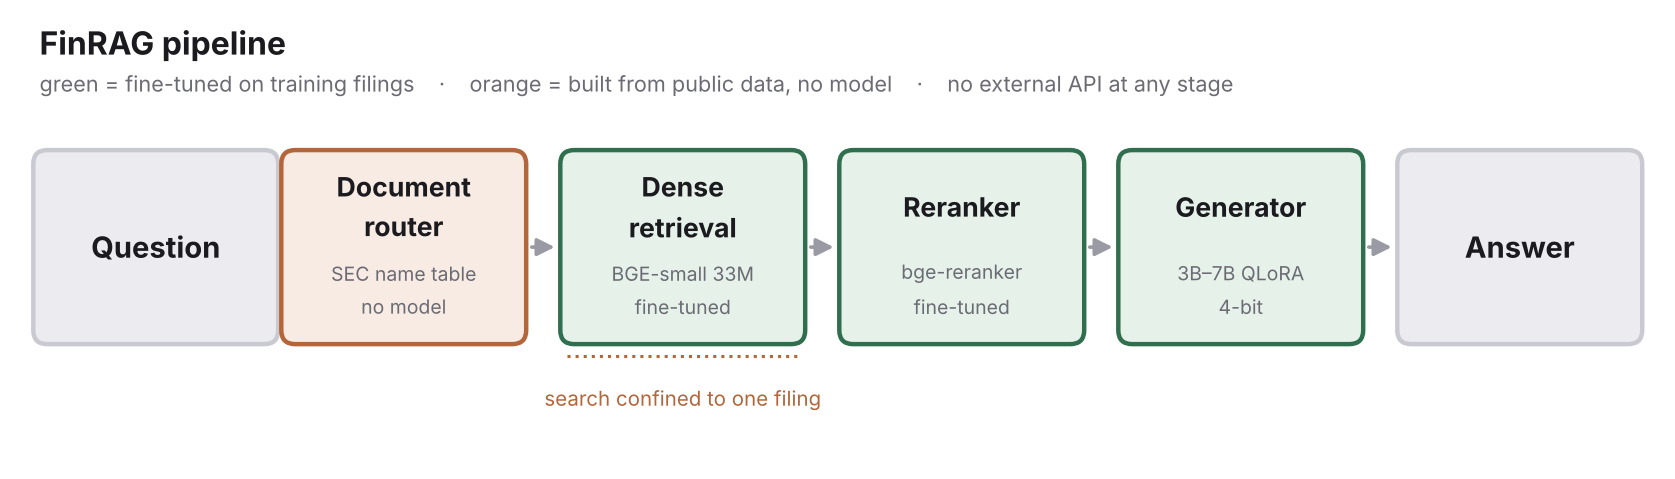
\includegraphics[width=\columnwidth]{fig5_pipeline.png}
\caption{The FinRAG pipeline. Shaded stages are fine-tuned on FinDER's training
filings; the router is constructed from public SEC data and is not learned.}
\label{fig:pipeline}
\end{figure}

\subsection{Embedding fine-tuning}
The first-stage retriever is \texttt{bge-small-en-v1.5}~\cite{xiao2023bge} (33M
parameters), fine-tuned with Multiple Negatives Ranking Loss. For a query
$q_i$ with positive $p_i^{+}$, cosine similarity $s(\cdot,\cdot)$ and
temperature $\tau$,
\begin{equation}
\mathcal{L}_i = -\log \frac{\exp\!\big(s(q_i, p_i^{+})/\tau\big)}
{\sum_{j} \exp\!\big(s(q_i, p_j)/\tau\big)} .
\end{equation}

Two details materially affected results. Positives are drawn from grade-2
chunks rather than arbitrarily, since an arbitrary choice frequently selects a
supporting fragment instead of the passage that actually answers the question.
Negatives are drawn under an exclusion band: labelled gold, the immediate
neighbours of gold chunks (which share overlap tokens by construction), and any
candidate whose content overlap with the gold text exceeds 0.35 are all
excluded, because training the model to push away text it should retrieve is
actively harmful. We mine four in-filing and four cross-filing negatives per
query; in-filing negatives teach fine-grained relevance, cross-filing negatives
teach company discrimination.

\subsection{Reranker fine-tuning}
The reranker is \texttt{bge-reranker-base}, trained on (query, positive,
negative) pairs with binary cross-entropy. Negatives must be mined from the
\emph{fine-tuned} retriever: the reranker sees that retriever's candidates at
inference, and training on easier base-model negatives leaves it unprepared.
Passages are clipped in the reranker's own tokenizer (XLM-RoBERTa) to 460
tokens, matching training exactly --- our 448-BGE-token chunks measure a mean
of 475 tokens under that tokenizer, so roughly 15\% would otherwise lose their
tail at inference.

\subsection{Document routing without an LLM}
\label{sec:routing}
Only about 11\% of the fine-tuned retriever's top-100 come from the question's
own filing: 10-K filings are structurally near-identical, so most retrieved
text is simply the wrong company. Restricting the candidate pool to one filing
is therefore the single largest available improvement, and HDRR reaches the
same conclusion, implementing it with one LLM call per query to extract the
ticker.

We implement it without a model. A first version matched capitalized tokens
against corpus tickers and routed when exactly one matched, which covers 78.4\%
of queries. It fails three ways: questions naming a company rather than a
ticker (``Div policy of Intuit\ldots''); collisions in which a financial
acronym is also a ticker, so a query that \emph{did} name its ticker is
discarded as ambiguous (``Growth acceleration in SNPS Design IP segment''
matches both SNPS and International Paper); and single-letter tickers, which a
2--6 character pattern cannot admit without catastrophic false positives.

Our router resolves these with a dictionary built from SEC's public
\texttt{company\_tickers.json}, restricted to the 497 corpus filings and
normalized into name variants, plus a stoplist of financial acronyms that are
also tickers. Evidence is ranked: an unambiguous ticker token wins outright,
because on this corpus a unique ticker names the correct filing 100\% of the
time, against 97.4\% for a name match; a company name is used only when no
unambiguous ticker is present. Where neither resolves, the query stays
unrouted and falls back to full-corpus retrieval, which is deliberately
conservative --- a wrong route confines retrieval to the wrong company with no
escape.

\subsection{Generator fine-tuning}
We fine-tune three instruction-tuned generators with QLoRA~\cite{dettmers2023qlora}
--- Qwen2.5-3B, Llama-3.2-3B and Mistral-7B-Instruct-v0.3 --- loading base
weights in 4-bit NF4 and training rank-16 adapters on attention and MLP
projections. Prompt tokens are masked so the loss is computed only on the
answer. Training examples pair a question with its gold context; 6\% are
abstention examples with deliberately varied refusal phrasings, since a
generator trained only on answerable questions will confabulate when retrieval
fails.

\section{Evaluation Protocol}
\label{sec:protocol}
Retrieval is scored with MRR@10, NDCG@10/@20 and Recall@$k$ against the graded
labels of Section~\ref{sec:data}, using linear gain $g/\log_2(r+1)$.
Generation is scored with ROUGE-L~\cite{lin2004rouge},
BLEU~\cite{papineni2002bleu}, BERTScore-F1~\cite{zhang2020bertscore}, and a
rounding-aware numeric exact-match on the subset of questions whose gold answer
contains a verifiable figure. All confidence intervals come from a paired
bootstrap with resampling indices shared across systems, so that per-system
intervals and pairwise differences are drawn from the same resamples;
independent per-system bootstraps ignore that every system is scored on the
same queries and overstate uncertainty on a difference.

\subsection{Comparison against HDRR}
\label{sec:protocol-hdrr}
HDRR's repository publishes per-query judge scores for every system in their
paper, keyed on FinDER question identifiers. This permits a comparison far
stronger than placing two aggregate numbers side by side, provided three
conditions hold.

\textbf{No leakage.} Their query splits draw from all 497 filings, 392 of which
trained our models. We therefore restrict to the intersection of their
published splits with our 98 held-out filings: 258 questions with recoverable
ground truth. Across all seven of their systems, scores on this subset fall
within $\pm0.3$ of their scores on their full query set, so the subset is not
an unrepresentative slice.

\textbf{Identical grading.} We reproduce their harness exactly: model
\texttt{gpt-4.1}, temperature 0, 100 max tokens, JSON-constrained output, their
\texttt{BENCHMARK\_EVALUATION} system and user prompts verbatim, and their
score parser. Ground truth is read from their own result files rather than
re-derived from the dataset, and we replicate their text sanitizer, so the
judge receives byte-identical references to the ones their judge received.

\textbf{Validated grader.} Before comparing, we re-scored 40 of HDRR's own
published answers with our harness. Agreement with their published scores was
90.0\% exact, 100\% within one point, mean difference $+0.05$, $r=0.993$. This
establishes that any difference we report is a difference between pipelines and
not between grading setups, and it bounds judge drift between their evaluation
and ours.

\section{Results}
\label{sec:results}

\subsection{Retrieval}
Table~\ref{tab:retrieval} reports retrieval on the 1{,}088 held-out questions.
Fine-tuning the 33M embedder more than doubles NDCG@10 over the strongest
off-the-shelf baseline (0.1866 versus 0.0777, $+0.1091$, CI
$[+0.0903,+0.1287]$). Document routing is the dominant single factor,
$+0.3468$ (CI $[+0.3269,+0.3691]$), and replacing the ticker regex with the SEC
dictionary router adds a further $+0.0580$ (CI $[+0.0460,+0.0705]$). Fig.~\ref{fig:retrieval} shows the progression. The
complete pipeline reaches NDCG@10 0.5994, a $16\times$ improvement over BM25
and $3.2\times$ over the fine-tuned dense retriever alone.

\begin{table}[t]
\caption{Retrieval on 1{,}088 held-out questions from 98 filings never seen in
training. Retrieval searches the full 181{,}867-chunk corpus; the final row is
the configuration carried into Table~\ref{tab:vshdrr}. FT = fine-tuned.}
\label{tab:retrieval}
\centering
\footnotesize
\setlength{\tabcolsep}{4pt}
\begin{tabular}{lcccc}
\toprule
System & NDCG@10 & MRR@10 & R@10 & R@100 \\
\midrule
BM25 & 0.0359 & 0.0403 & 0.0613 & 0.1742 \\
BGE-base, off the shelf & 0.0681 & 0.0727 & 0.1030 & 0.2304 \\
BGE-small, off the shelf & 0.0777 & 0.0807 & 0.1134 & 0.2256 \\
\midrule
FT dense & 0.1866 & 0.1994 & 0.2420 & 0.4032 \\
FT dense + RRF & 0.1678 & 0.1739 & 0.2451 & 0.4033 \\
FT dense + ticker route & 0.5342 & 0.5354 & 0.7021 & 0.8801 \\
\quad + FT reranking & 0.5414 & 0.5550 & 0.6706 & 0.8368 \\
\textbf{\quad + SEC-name route} & \textbf{.5994} & \textbf{.6171} & \textbf{.7322} & \textbf{.8749} \\
\bottomrule
\end{tabular}
\end{table}

Two negative results are worth recording. Sparse fusion \emph{hurts} once the
embedder is domain-adapted ($-0.0189$, CI $[-0.0314,-0.0056]$). And reranking
applied to unrouted candidates is sharply harmful ($-0.1021$, CI
$[-0.1211,-0.0841]$), while the same reranker applied \emph{after} routing is
mildly positive but not significant ($+0.0075$, CI $[-0.0156,+0.0297]$). A
reranker trained on one candidate distribution and deployed on another
mis-ranks; the component is not independently useful, only useful in position.

\begin{figure}[t]
\centering
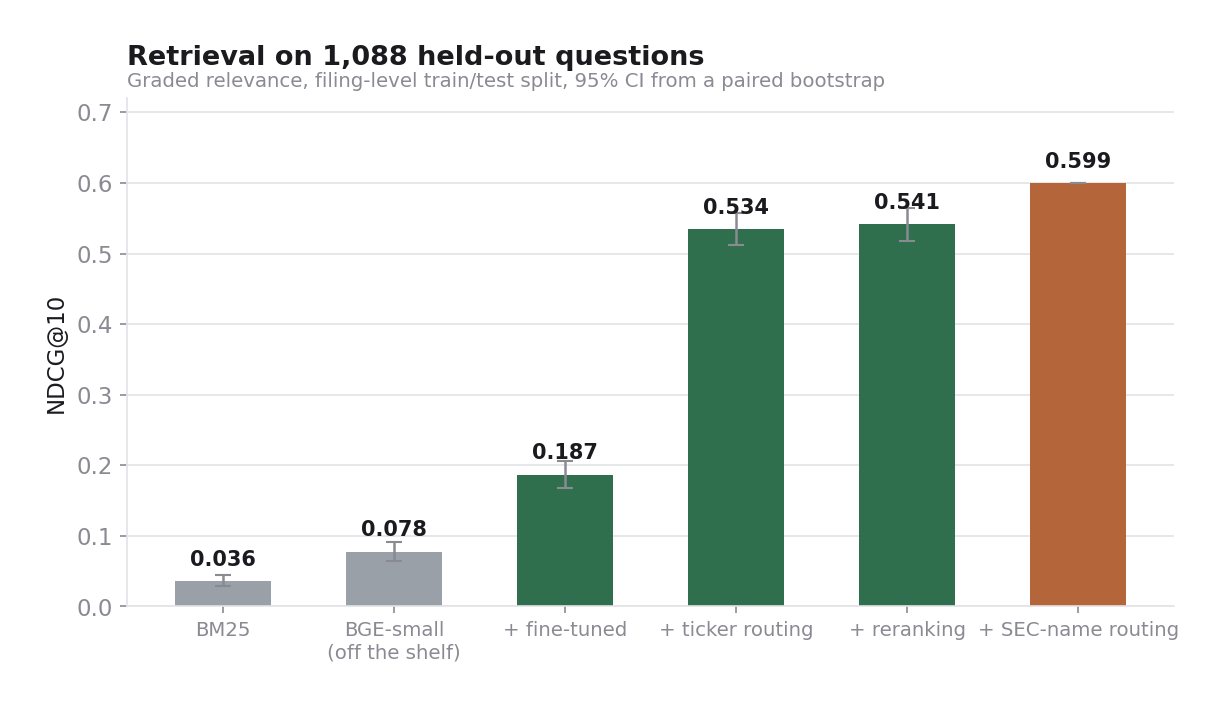
\includegraphics[width=\columnwidth]{04_retrieval.png}
\caption{Retrieval on 1{,}088 held-out questions. Error bars are 95\% paired
bootstrap intervals. Document routing, not reranking, is the dominant factor.}
\label{fig:retrieval}
\end{figure}

\subsection{Document routing}
Table~\ref{tab:router} and Fig.~\ref{fig:router} compare the three routers on the 259 queries shared
with HDRR, scored against the filing our labels place the gold chunks in. The
SEC dictionary recovers two thirds of the gap between the regex and HDRR's LLM
router at no inference cost. More tellingly, on the 232 queries where both our
router and theirs commit to a filing, they select the \emph{same} filing 232
times --- the two methods are not approximating each other, they agree
exactly. The residual difference is coverage, not correctness: HDRR commits on
17 queries where we abstain.

\begin{table}[t]
\caption{Document routing on the 259 shared queries. ``Correct'' is the share of
all queries routed to the filing containing the gold evidence.}
\label{tab:router}
\centering
\footnotesize
\setlength{\tabcolsep}{4pt}
\begin{tabular}{lcccc}
\toprule
Router & Cost/query & Routed & Prec. & Correct \\
\midrule
HDRR, LLM extraction & 1 call & 96.1\% & 98.8\% & \textbf{95.0\%} \\
Ours, ticker regex & none & 78.0\% & 100.0\% & 78.0\% \\
\textbf{Ours, SEC names} & \textbf{none} & 90.3\% & 98.7\% & 89.2\% \\
\bottomrule
\end{tabular}
\end{table}

\begin{figure}[t]
\centering
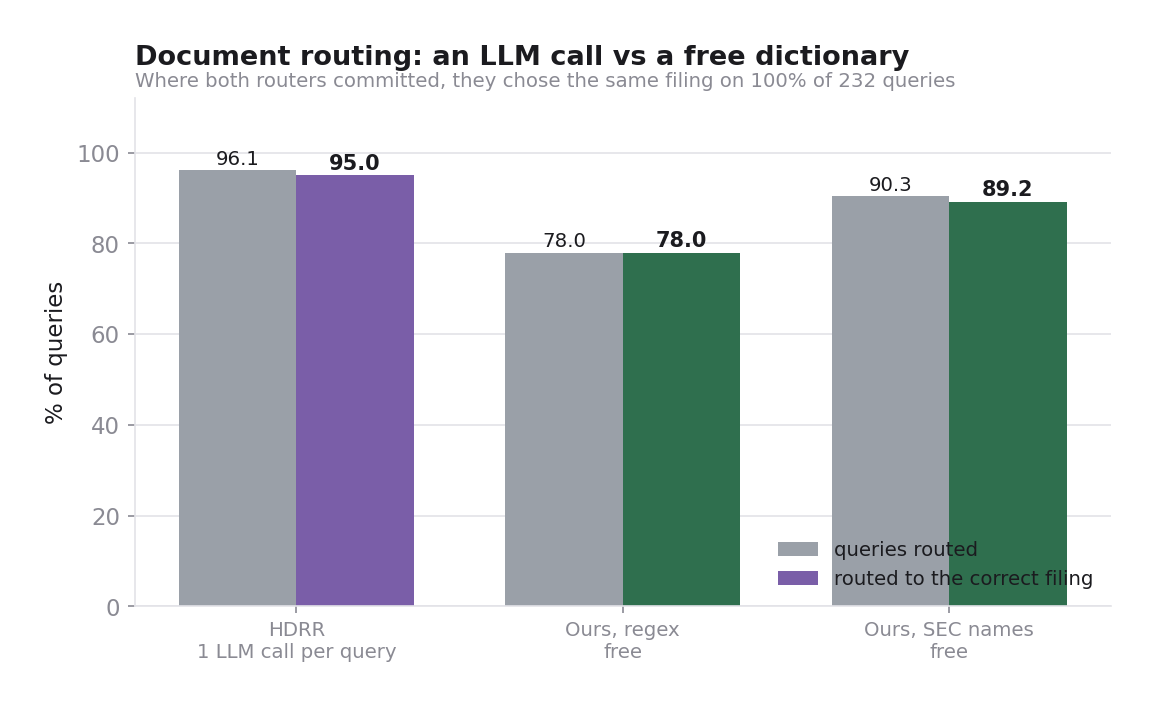
\includegraphics[width=\columnwidth]{05_router.png}
\caption{Document routing: one LLM call per query against a free dictionary
lookup. Where both routers commit to a filing, they choose the same one on
100\% of 232 queries.}
\label{fig:router}
\end{figure}

\subsection{Generator selection}
\label{sec:genselect}
Table~\ref{tab:generation} reports the three fine-tuned generators on the
held-out questions, under retrieved context and under gold context. This
experiment selected the generator used in the rest of the paper, and was
therefore run before the routing improvement of Section~\ref{sec:routing}
existed: it uses ticker-regex routing at context depth 3, whereas the
system evaluated in Section~\ref{sec:vshdrr} uses SEC-name routing at depth
10. All three models are compared under identical conditions, so the ranking
between them is unaffected; the newer pipeline would raise the retrieved rows
by roughly 0.01 ROUGE-L without reordering them. We report the selection
configuration rather than restating it under the final one, since the choice
was made on these numbers.

QLoRA raises ROUGE-L by 20--24\% relative over the corresponding base model
for every backbone. Mistral-7B is strongest on surface overlap; Qwen2.5-3B is
strongest on numeric exact-match despite being less than half the size, which
suggests numeric fidelity and fluency are not the same capability. We take
Mistral-7B forward on that basis.

\begin{table}[t]
\caption{Generator selection on held-out questions, under
\textbf{ticker-regex routing at context depth 3} (see
Section~\ref{sec:genselect}). Numeric EM is computed on the trusted numeric
subset ($n=121$) with a rounding-aware criterion.}
\label{tab:generation}
\centering
\small
\begin{tabular}{llccc}
\toprule
Generator & Context & ROUGE-L & BERTScore & Num.\ EM \\
\midrule
Qwen2.5-3B & retrieved & 0.2041 & 0.8626 & 0.107 \\
Llama-3.2-3B & retrieved & 0.2119 & 0.8644 & 0.083 \\
Mistral-7B & retrieved & \textbf{0.2318} & \textbf{0.8712} & 0.099 \\
\midrule
Qwen2.5-3B & gold & 0.2229 & 0.8704 & \textbf{0.190} \\
Llama-3.2-3B & gold & 0.2312 & 0.8712 & 0.091 \\
Mistral-7B & gold & \textbf{0.2518} & \textbf{0.8783} & 0.140 \\
\bottomrule
\end{tabular}
\end{table}

\subsection{Comparison with HDRR}
\label{sec:vshdrr}
Table~\ref{tab:vshdrr} and Fig.~\ref{fig:deltas} report the paired comparison under the protocol of
Section~\ref{sec:protocol-hdrr}. FinRAG scores 6.02 against HDRR's 7.63. The
difference is real and we report it as such: the 95\% CI is
$[-2.08,-1.13]$ and excludes zero. FinRAG is statistically indistinguishable
from their Agentic RAG configuration and loses to the remaining three.

\begin{table}[t]
\caption{Paired comparison on 258 shared held-out queries, scored by HDRR's own
GPT-4.1 judge with their rubric and prompt. FinRAG here is the final system:
\textbf{SEC-name routing at context depth 10}. CIs from 10{,}000 paired
bootstrap resamples. $\Delta$ is ours minus theirs; W/L/T counts queries where
our score was strictly higher, strictly lower, or equal.}
\label{tab:vshdrr}
\centering
\footnotesize
\setlength{\tabcolsep}{4pt}
\begin{tabular}{lcccc}
\toprule
System & Mean & $\Delta$ & 95\% CI & W/L/T \\
\midrule
HDRR & 7.63 & $-1.61$ & $[-2.08,-1.13]$ & 58/145/55 \\
CBR + LLM route & 7.44 & $-1.41$ & $[-1.91,-0.92]$ & 69/141/48 \\
CBR + metadata & 6.84 & $-0.82$ & $[-1.32,-0.32]$ & 75/133/50 \\
Unnamed base & 6.61 & $-0.59$ & $[-1.04,-0.12]$ & 102/105/51 \\
Agentic RAG & 6.27 & $-0.25$ & $[-0.78,+0.30]$ & 101/118/39 \\
\midrule
\textbf{FinRAG (ours)} & \textbf{6.02} & --- & --- & --- \\
\bottomrule
\end{tabular}
\end{table}

\begin{figure}[t]
\centering
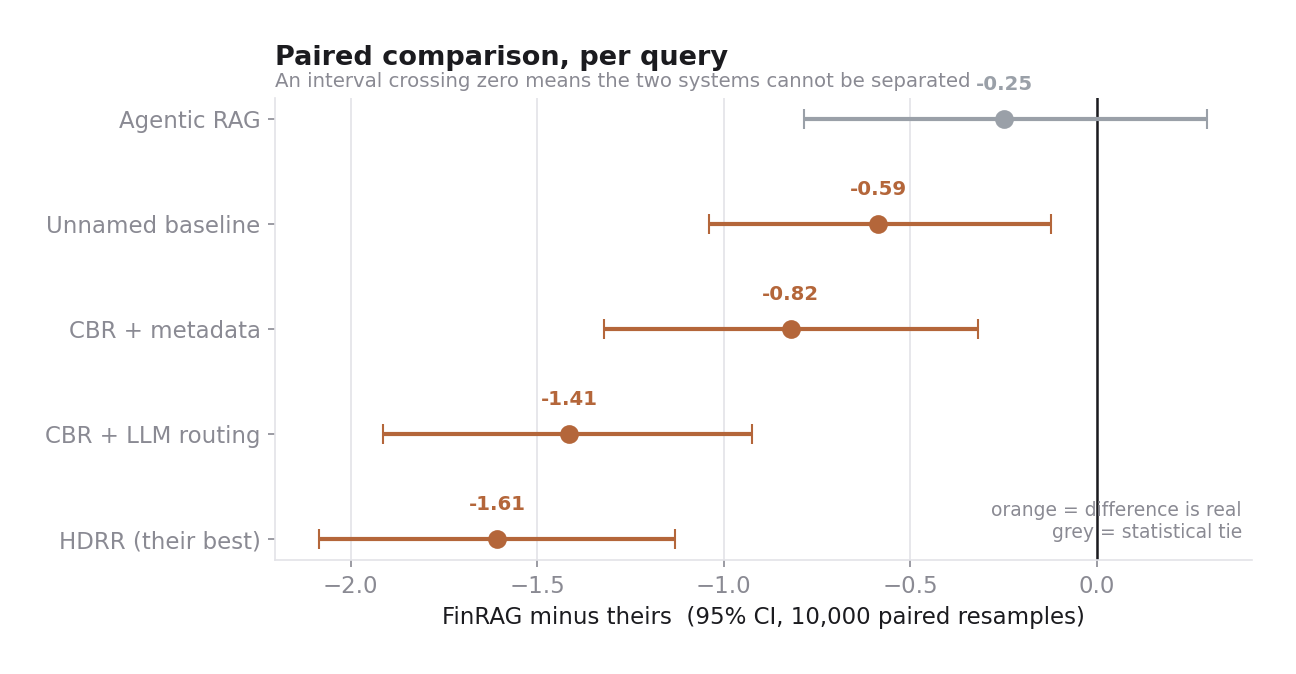
\includegraphics[width=\columnwidth]{02_deltas.png}
\caption{Paired per-query differences against each published system, with 95\%
bootstrap intervals. An interval crossing zero means the two systems cannot be
separated on these queries.}
\label{fig:deltas}
\end{figure}

\subsection{Where the gap comes from}
\label{sec:decomp}
The value of measuring both stages is that the deficit can be attributed.
Supplying the same generator with gold evidence instead of retrieved context
raises its judged score from 6.02 to 6.70 (Fig.~\ref{fig:decomp}). The 1.61-point gap therefore
decomposes as
\begin{equation}
\underbrace{0.67}_{\text{retrieval}} + \underbrace{0.93}_{\text{generator}} =
1.61 ,
\end{equation}
\begin{figure}[t]
\centering
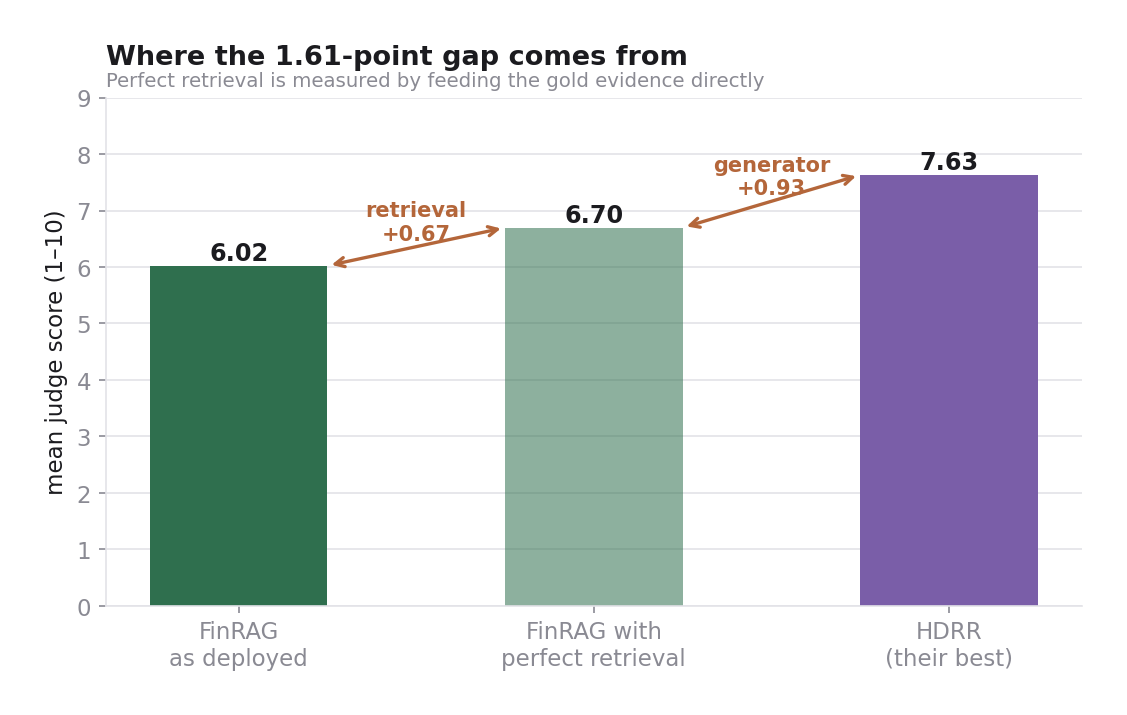
\includegraphics[width=\columnwidth]{03_decomposition.png}
\caption{Decomposition of the 1.61-point deficit. The middle bar supplies the
same generator with gold evidence, isolating retrieval loss from generator
capacity.}
\label{fig:decomp}
\end{figure}

and the two halves have different character. The retrieval component is a
property of our pipeline and is addressable: 37\% of queries receive no gold
chunk in their top-3 context, and deepening the context window from 3 to 10
passages recovers part of it. The generator component is a property of the
hardware budget: HDRR's answers are produced by a frontier API model, ours by a
4-bit 7B model on a laptop. At the retrieval ceiling, FinRAG is statistically
indistinguishable from three of HDRR's five published configurations.

A further observation supports this reading. HDRR's scores are essentially flat
with respect to \emph{our} retrieval outcome --- 7.54 on queries where our
retriever found gold, 7.81 where it did not. The queries we fail are not
intrinsically hard; a sufficiently strong generator compensates for weaker
evidence. This is also a caution about the metric: an end-to-end judged score
is relatively insensitive to retrieval quality, which is precisely why
retrieval should be reported separately.

\subsection{Efficiency}
Table~\ref{tab:efficiency} reports the deployed cost. The entire pipeline fits
in 5.3--7.3\,GB of VRAM. Retrieval and routing together account for
approximately 0.5\,s of a 12--15\,s query; generation dominates. Notably,
vocabulary size rather than parameter count drives memory and speed:
Qwen2.5-3B, with a 152k vocabulary, is both heavier and slower than Mistral-7B
with a 33k vocabulary.

\begin{table}[t]
\caption{Deployed cost on one RTX~4080 Laptop GPU (12.9\,GB), 50 queries, full
pipeline co-resident. No external API calls at any stage.}
\label{tab:efficiency}
\centering
\small
\begin{tabular}{lccc}
\toprule
Generator & Peak VRAM & Tokens/s & Median latency \\
\midrule
Llama-3.2-3B & 5.32\,GB & 13.2 & 12.0\,s \\
Qwen2.5-3B & 6.30\,GB & 9.6 & 15.0\,s \\
Mistral-7B & 7.27\,GB & 11.4 & 14.3\,s \\
\bottomrule
\end{tabular}
\end{table}

\section{Discussion}
\label{sec:disc}

\textbf{Routing dominates, and it does not need a model.} The largest single
retrieval gain in this work, $+0.3468$ NDCG@10, comes from confining search to
one filing. HDRR reaches the same architectural conclusion and pays an LLM call
per query for it. Our dictionary router reaches 89.2\% correct routing against
their 95.0\%, and agrees with their decision on 100\% of queries where both
commit. For a corpus with a closed, enumerable entity set --- which describes
most regulatory filing collections --- entity routing appears to be a lookup
problem that has been treated as an inference problem.

\textbf{Component quality is positional, not intrinsic.} Our reranker degrades
NDCG@10 by 0.10 when applied to unrouted candidates and helps marginally when
applied after routing. Sparse fusion helps a generic embedder and hurts a
domain-adapted one. Neither component has a fixed value; both are functions of
the candidate distribution they see. Reporting a reranker's contribution
without specifying what precedes it is therefore not very informative.

\textbf{Abstention is penalised by construction.} HDRR's rubric instructs the
judge to score 1--3 when an answer states the information could not be found,
regardless of whether refusing was correct. Our generator is deliberately
calibrated to abstain, and does so on 6.6\% of queries; excluding those raises
our mean from 6.02 to 6.34. We report the penalised figure as the headline
because it is the one measured under their protocol, but note that a rubric
which punishes calibrated refusal as harshly as confident fabrication rewards a
behaviour most financial deployments would not want. Supporting evidence: our
abstention rate falls from 6.6\% to 4.3\% when gold evidence is supplied, so
the model abstains because context lacks the answer, not reflexively.

\textbf{What local actually costs.} On this benchmark the answer is 1.61 judged
points, of which 0.93 is attributable to generator capacity. In exchange, the
system runs in 7.3\,GB on a consumer laptop, makes no external calls, and sends
no filing text to a third party --- which, for regulated financial data, is
frequently a requirement rather than a preference.

\section{Limitations}
\label{sec:limits}
Our grader validation used 40 of HDRR's answers, which are predominantly
high-scoring (mean 7.95); it therefore establishes agreement in the upper range
more firmly than near our own operating point of 6.0. Relatedly, the judge
(GPT-4.1) and HDRR's generator come from the same model family, so
self-preference cannot be excluded as a contributor to the gap; we use their
judge deliberately, since a different judge would make the comparison
incommensurable with their published numbers, but the direction of any such
bias is unfavourable to us.

Their published scores were produced several months before ours. Our
replication bounds drift at $+0.05$ on 40 queries, but the two score sets are
not from a single judging run.

The generator-selection experiment of Section~\ref{sec:genselect} was run
under the pipeline as it stood at the time (ticker routing, depth 3), not
under the final configuration. The three generators are compared under
identical conditions there, so the selection itself is sound, but the
absolute values in Table~\ref{tab:generation} are not directly comparable to
the final system's. We estimate the final pipeline would raise those
retrieved rows by roughly 0.01 ROUGE-L.

Our relevance labels are induced rather than human-annotated. The coverage
criterion is conservative and will miss chunks that contain an answer without
reproducing the reference wording; an observed consequence is that queries
whose labelled gold was never retrieved still improved when given more context,
implying our NDCG understates true retrieval quality to some degree.

Finally, we compare against HDRR on judged answer quality only. Their paper
reports no retrieval metrics, and FinDER's own paper reports retrieval as RAGAS
Context Recall rather than rank-based measures, so our NDCG figures have no
published comparison point on this benchmark. Establishing one is the obvious
next step.

\section{Conclusion}
We built a financial RAG pipeline that runs entirely on a single 12\,GB
consumer GPU with no paid inference, and evaluated it against a published
API-based system under that system's own judge, rubric and prompt, after
demonstrating that our grading harness reproduces their published scores at
$r=0.993$. The local system scores 6.02 against 7.63 --- a real and reported
loss --- but the comparison decomposes it into 0.67 points of retrieval
deficit and 0.93 points of generator capacity, and shows that at the retrieval
ceiling the local pipeline is statistically indistinguishable from three of five
published configurations. Along the way we find that document routing, the
largest single retrieval factor, can be done by dictionary lookup rather than
by an LLM call, at exact agreement with the learned router wherever both
commit.

We suggest that the useful question for locally-hosted RAG is not whether it
beats a frontier-API system, but what the difference costs and where it lives.
Answering that requires reporting retrieval and generation separately, which
end-to-end judged evaluation does not do. Code, labels, run files and the
evaluation harness are
available.\footnote{\url{https://github.com/Haroon-M-Bilal/finrag-}}

\begin{thebibliography}{00}
\bibitem{lewis2020rag} P. Lewis \textit{et al.}, ``Retrieval-augmented generation for knowledge-intensive NLP tasks,'' in \textit{Proc. NeurIPS}, 2020.
\bibitem{karpukhin2020dpr} V. Karpukhin \textit{et al.}, ``Dense passage retrieval for open-domain question answering,'' in \textit{Proc. EMNLP}, 2020.
\bibitem{robertson2009bm25} S. Robertson and H. Zaragoza, ``The probabilistic relevance framework: BM25 and beyond,'' \textit{Found. Trends Inf. Retr.}, vol. 3, no. 4, 2009.
\bibitem{khattab2020colbert} O. Khattab and M. Zaharia, ``ColBERT: Efficient and effective passage search via contextualized late interaction over BERT,'' in \textit{Proc. SIGIR}, 2020.
\bibitem{reimers2019sbert} N. Reimers and I. Gurevych, ``Sentence-BERT: Sentence embeddings using Siamese BERT-networks,'' in \textit{Proc. EMNLP}, 2019.
\bibitem{izacard2022contriever} G. Izacard \textit{et al.}, ``Unsupervised dense information retrieval with contrastive learning,'' \textit{TMLR}, 2022.
\bibitem{wang2022e5} L. Wang \textit{et al.}, ``Text embeddings by weakly-supervised contrastive pre-training,'' \textit{arXiv:2212.03533}, 2022.
\bibitem{ni2022gtr} J. Ni \textit{et al.}, ``Large dual encoders are generalizable retrievers,'' in \textit{Proc. EMNLP}, 2022.
\bibitem{xiao2023bge} S. Xiao \textit{et al.}, ``C-Pack: Packed resources for general Chinese embeddings,'' \textit{arXiv:2309.07597}, 2023.
\bibitem{thakur2021beir} N. Thakur \textit{et al.}, ``BEIR: A heterogeneous benchmark for zero-shot evaluation of information retrieval models,'' in \textit{Proc. NeurIPS Datasets}, 2021.
\bibitem{nogueira2019passage} R. Nogueira and K. Cho, ``Passage re-ranking with BERT,'' \textit{arXiv:1901.04085}, 2019.
\bibitem{cormack2009rrf} G. V. Cormack, C. L. A. Clarke, and S. B\"uttcher, ``Reciprocal rank fusion outperforms Condorcet and individual rank learning methods,'' in \textit{Proc. SIGIR}, 2009.
\bibitem{gao2022hyde} L. Gao \textit{et al.}, ``Precise zero-shot dense retrieval without relevance labels,'' \textit{arXiv:2212.10496}, 2022.
\bibitem{hu2021lora} E. J. Hu \textit{et al.}, ``LoRA: Low-rank adaptation of large language models,'' \textit{arXiv:2106.09685}, 2021.
\bibitem{dettmers2023qlora} T. Dettmers \textit{et al.}, ``QLoRA: Efficient finetuning of quantized LLMs,'' in \textit{Proc. NeurIPS}, 2023.
\bibitem{qwen2024} Qwen Team, ``Qwen2.5 technical report,'' \textit{arXiv:2412.15115}, 2024.
\bibitem{touvron2023llama} H. Touvron \textit{et al.}, ``Llama 2: Open foundation and fine-tuned chat models,'' \textit{arXiv:2307.09288}, 2023.
\bibitem{jiang2023mistral} A. Q. Jiang \textit{et al.}, ``Mistral 7B,'' \textit{arXiv:2310.06825}, 2023.
\bibitem{araci2019finbert} D. Araci, ``FinBERT: Financial sentiment analysis with pre-trained language models,'' \textit{arXiv:1908.10063}, 2019.
\bibitem{wu2023bloomberggpt} S. Wu \textit{et al.}, ``BloombergGPT: A large language model for finance,'' \textit{arXiv:2303.17564}, 2023.
\bibitem{chen2021finqa} Z. Chen \textit{et al.}, ``FinQA: A dataset of numerical reasoning over financial data,'' in \textit{Proc. EMNLP}, 2021.
\bibitem{finder2025} Linq AI Research, ``FinDER: Financial dataset for question answering and evaluating retrieval-augmented generation,'' \textit{arXiv:2504.15800}, 2025.
\bibitem{es2023ragas} S. Es \textit{et al.}, ``RAGAS: Automated evaluation of retrieval augmented generation,'' \textit{arXiv:2309.15217}, 2023.
\bibitem{lin2004rouge} C.-Y. Lin, ``ROUGE: A package for automatic evaluation of summaries,'' in \textit{Proc. ACL Workshop}, 2004.
\bibitem{papineni2002bleu} K. Papineni \textit{et al.}, ``BLEU: A method for automatic evaluation of machine translation,'' in \textit{Proc. ACL}, 2002.
\bibitem{zhang2020bertscore} T. Zhang \textit{et al.}, ``BERTScore: Evaluating text generation with BERT,'' in \textit{Proc. ICLR}, 2020.
\bibitem{zheng2023judge} L. Zheng \textit{et al.}, ``Judging LLM-as-a-judge with MT-Bench and Chatbot Arena,'' in \textit{Proc. NeurIPS Datasets}, 2023.
\bibitem{basepaper2026} Y. Cheng \textit{et al.}, ``Enhancing financial report question-answering: A retrieval-augmented generation system with reranking analysis,'' \textit{arXiv:2603.16877}, 2026.
\bibitem{hdrr2026} Y. Cheng, Lai, and Liu, ``Sustainable hybrid document-routed retrieval for financial RAG,'' \textit{Intelligent Systems with Applications}, vol. 32, art. 200720, 2026.
\end{thebibliography}

\end{document}
